\chapter {Thiết kế và xây dựng hệ thống}

\section{Tổng quan về kiến trúc hệ thống }

Kiến trúc phần cứng của hệ thống robot bốn chân được xây dựng nhằm mục tiêu cung cấp nguồn năng lượng ổn định, đảm bảo khả năng xử lý thuật toán phức tạp theo thời gian thực và điều khiển đồng bộ nhiều cơ cấu chấp hành. Sơ đồ kết nối phần cứng tổng thể của mô hình thực nghiệm được thể hiện chi tiết trong Hình~\ref{fig30}.

\begin{figure}[H]
    \centering
    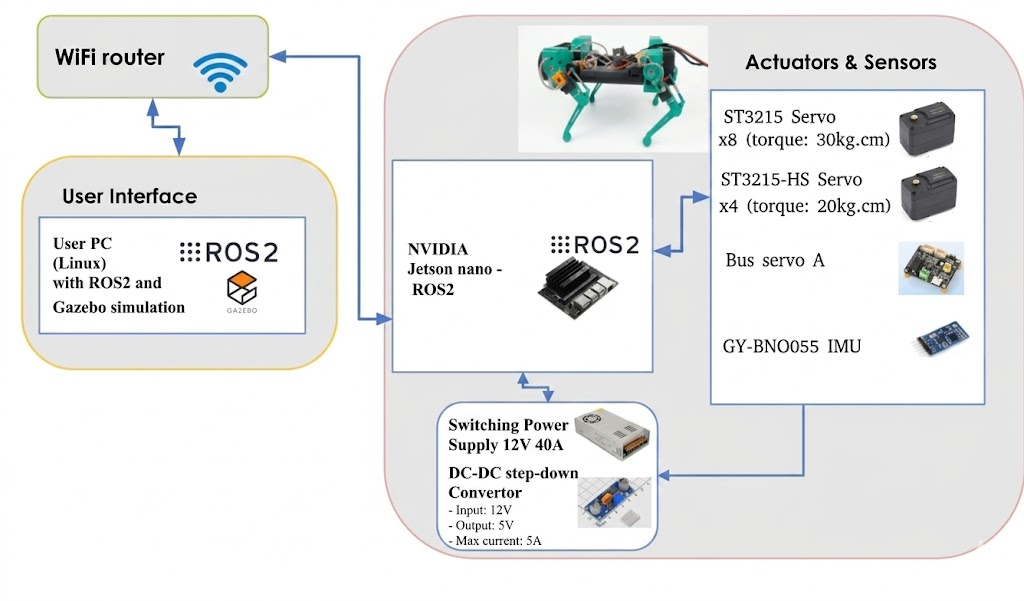
\includegraphics[width=\textwidth]{img/fig_system_overview_new.png}
    \caption{Sơ đồ kiến trúc tổng thể của hệ thống robot bốn chân.}
    \label{fig30}
\end{figure}

Hình~\ref{fig:real_robot} trình bày mô hình robot bốn chân thực tế đã được chế tạo và lắp ráp hoàn chỉnh. Robot sử dụng khung thân và các chi tiết chân được gia công bằng công nghệ in 3D FDM với vật liệu PLA, tích hợp 12 động cơ bus servo ST3215 tại các khớp, cảm biến IMU BNO055 gắn trên thân và máy tính nhúng Jetson Nano làm bộ xử lý trung tâm.

\begin{figure}[H]
    \centering
    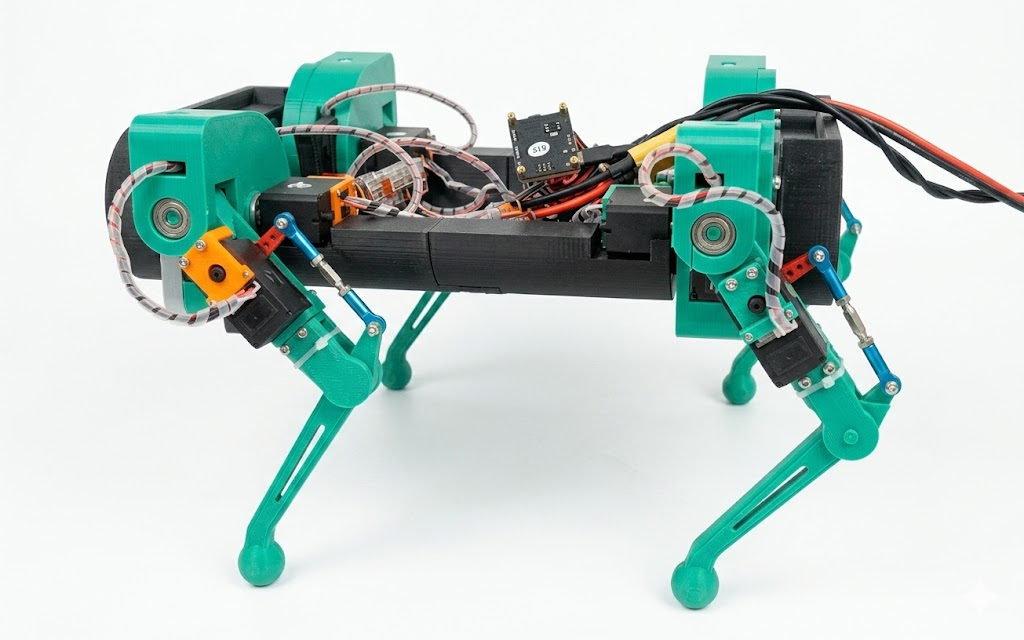
\includegraphics[width=0.85\textwidth]{img/fig_real_robot.png}
    \caption{Mô hình robot bốn chân thực tế đã được chế tạo và lắp ráp hoàn chỉnh.}
    \label{fig:real_robot}
\end{figure}

\subsection{Khối xử lý trung tâm }
Một yếu tố quan trọng của nguyên mẫu này là bộ xử lý trung tâm. Điều đầu tiên cần giải quyết là khả năng tính toán các bài toán phức tạp như động học nghịch, quy hoạch quỹ đạo và xử lý dữ liệu cân bằng theo thời gian thực.

Nhóm đã quyết định sử dụng máy tính nhúng Jetson Nano Developer Kit B01 \cite{jetson_nano} thay vì các dòng vi điều khiển phổ thông vì nó mang lại sức mạnh tính toán vượt trội hơn hẳn. Những ưu điểm này bao gồm: tốc độ xung nhịp cao từ vi xử lý Quad-core ARM Cortex-A57, tích hợp GPU mạnh mẽ, khả năng chạy hệ điều hành Linux (Ubuntu) hỗ trợ đa nhiệm, và dễ dàng tích hợp các thư viện toán học phức tạp. Nhược điểm chính của nền tảng tiên tiến này là mức tiêu thụ điện năng lớn hơn và độ phức tạp trong việc làm chủ hệ thống phần mềm.


\begin{figure}[H]
    \centering
    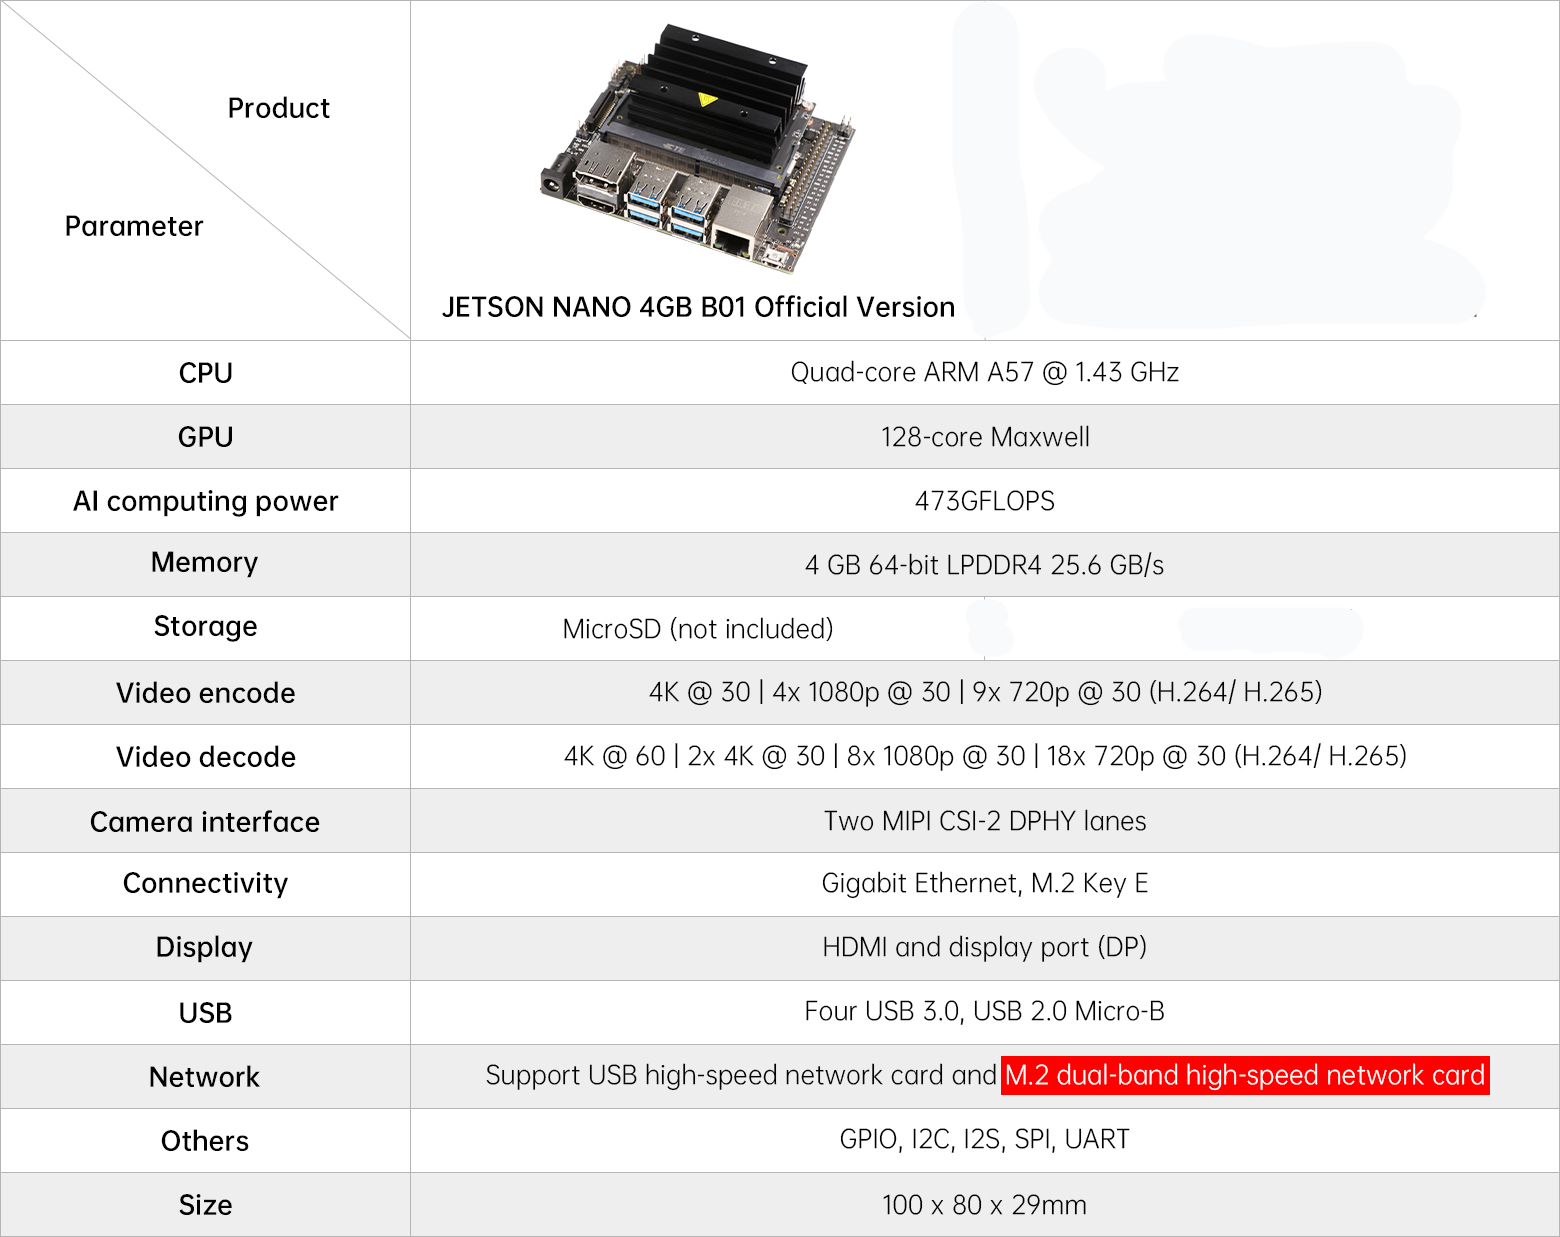
\includegraphics[width=0.8\textwidth]{img/fig34-Specifications-Jetson-B01.png} 
    \caption{Thông số kỹ thuật Jetson Nano B01}
    \label{fig34}
    \vspace{0.2cm}
\end{figure}

Hầu hết những người chế tạo robot giải trí đơn giản thường sử dụng vi điều khiển Arduino. Tuy nhiên, trong các hệ thống robot đa chân đòi hỏi khả năng giữ thăng bằng động và xử lý toán học ma trận tốc độ cao, các máy tính nhúng như dòng Jetson lại là tiêu chuẩn trong nhiều nguyên mẫu nghiên cứu. Chúng được sử dụng trong nhiều lĩnh vực, từ robot tự hành (AMR), xe tự lái đến các hệ thống AI xử lý tại biên (Edge AI) đắt tiền. Tất cả những yếu tố này đã ảnh hưởng đến quyết định của chúng em khi lựa chọn bộ xử lý cấp cao hơn cho dự án.

Jetson Nano được sử dụng để điều khiển nguyên mẫu của chúng em, bao gồm việc quản lý 12 động cơ servo và đọc dữ liệu từ module cảm biến IMU. Jetson Nano thiết lập giao tiếp UART với hai mạch Bus Servo Adapter (A). Hai mạch chuyển đổi này sẽ nhận các gói tin lệnh từ Jetson Nano và phân phối tín hiệu điều khiển nối tiếp đến 12 động cơ servo (mỗi mạch quản lý một nửa số lượng servo). Cấu trúc này giúp giảm tải dòng điện qua mạch điều khiển, phân bổ công suất hợp lý và tối giản hóa việc đi dây vật lý cho hai nửa của robot. 

\subsection{ Hệ thống Cung cấp Nguồn điện}

Sau khi nghiên cứu và lựa chọn động cơ servo ST3215 cùng mạch điều khiển, việc cấp nguồn đúng cách để hệ thống có thể đáp ứng các yêu cầu khắt khe về dòng điện tức thời trở nên vô cùng quan trọng. Để đạt được mục tiêu này, nhóm bắt đầu xem xét các phương án cung cấp năng lượng khác nhau, bao gồm pin và nguồn cấp điện trực tiếp. Các thông số kỹ thuật cốt lõi được đặt ra cho dự án bao gồm: Điện áp hoạt động, Dòng điện tối đa, Công suất tổng và Độ ổn định điện áp. Hai phương án chính được đưa ra cân nhắc là sử dụng Pin Lithium Polymer dung lượng lớn và Nguồn xung tổ ong; mỗi loại đều có những đặc tính riêng tác động đến quá trình thử nghiệm.

Trong giai đoạn phát triển, thử nghiệm thuật toán và tinh chỉnh động học, hệ thống yêu cầu một nguồn điện có khả năng cung cấp dòng xả lớn, liên tục trong nhiều giờ đồng hồ mà không xảy ra hiện tượng sụt áp. Việc khởi chạy hoặc ép tải 12 động cơ servo cùng lúc đòi hỏi dòng khởi động cực kỳ cao. Do đó, nguồn xung tổ ong 12V - 40A (480W) đã được lựa chọn làm giải pháp cung cấp năng lượng chính thay vì dùng pin. Ưu điểm lớn nhất của nguồn tổ ong là giá thành hợp lý, khả năng cấp dòng xả lên đến 40A một cách ổn định và cung cấp đúng mức điện áp 12V tối ưu cho các servo ST3215 hoạt động với hiệu suất cao nhất. 

\begin{figure}[H]
    \centering
    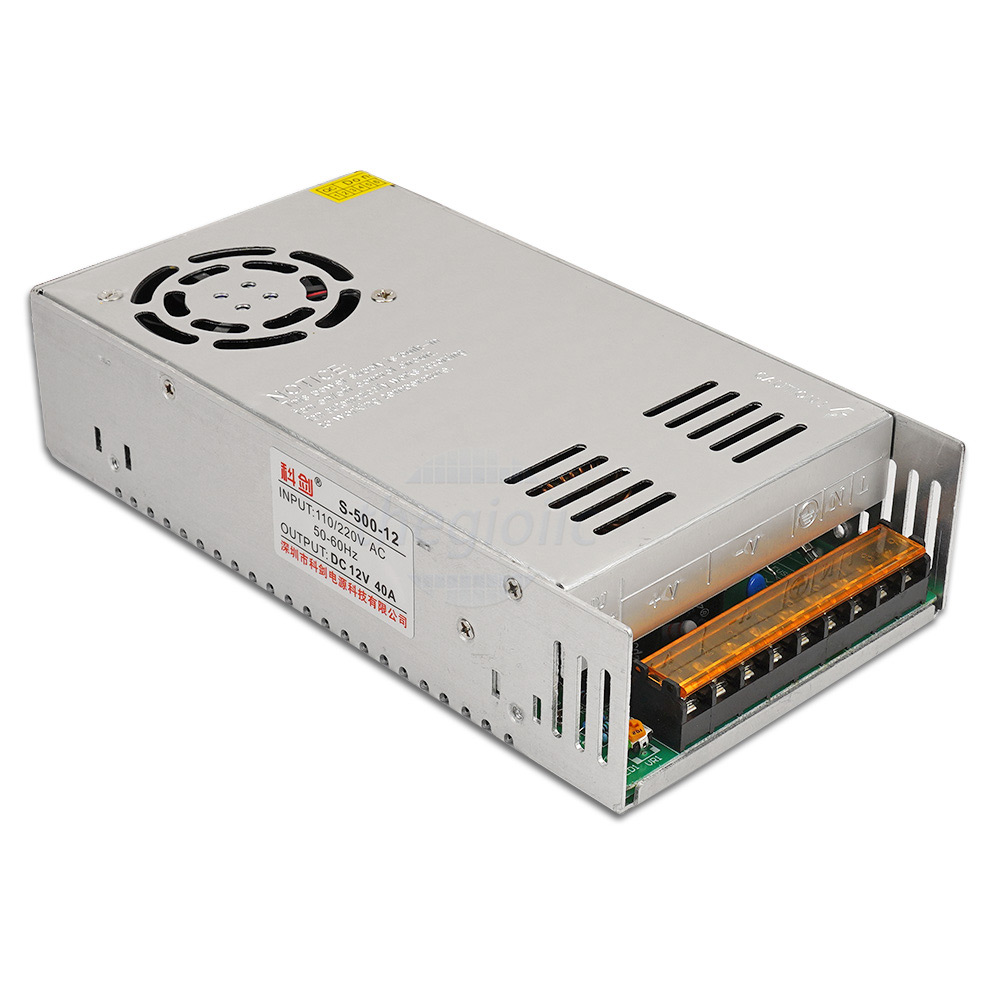
\includegraphics[width=0.6\textwidth]{img/fig35-Nguồn Xung Tổ Ong 12V 40A 480W.png} 
    \caption{Bộ nguồn xung tổ ong 12V 40A 480W}
    \label{fig35}
    \vspace{0.2cm}
\end{figure}

Việc lựa chọn nguồn xung tổ ong 12V - 40A (480W) được dựa trên tính toán dòng điện tiêu thụ của 12 động cơ servo ST3215:

Dòng điện không tải/hoạt động bình thường : Khoảng 300mA - 600mA / servo (tại 12V).
    
Dòng điện khởi động/giữ tải lớn nhất ($I_{stall}$): Khoảng 2.7A / servo (tại 12V).

Trong trường hợp xấu nhất khi robot khởi động hoặc thực hiện động tác nâng toàn thân, giả sử cả 12 servo đều chịu tải lớn, tổng dòng điện tức thời ($I_{total}$) là:

$$I_{total} = N_{servo} \times I_{stall} = 12 \times 2.7 = 32.4A$$

Theo đó, tổng công suất tiêu thụ điện tối đa ($P_{total}$) của riêng hệ thống cơ cấu chấp hành là:

$$P_{total} = I_{total} \times U = 32.4 \times 12 = 388.8W$$

Để đảm bảo an toàn và tuổi thọ cho linh kiện, tránh sụt áp nguồn khi ép tải, hệ số an toàn ($k$) thường được chọn từ 1.2 đến 1.5. Ở đây nhóm chọn hệ số $k = 1.2$, ta có yêu cầu công suất nguồn cấp tối thiểu phải đạt:

$$P_{source} \ge P_{total} \times k = 388.8 \times 1.2 = 466.56W$$

Việc lựa chọn nguồn xung tổ ong 12V - 40A (công suất cực đại 480W) là hoàn toàn chính xác và bám sát với tính toán lý thuyết ($466.56W \le 480W$). Mức công suất và dòng điện này đảm bảo khả năng đáp ứng dòng xả cao ngay cả khi robot hoạt động ở trạng thái tải nặng nhất mà không gây sụt áp hệ thống, giúp vi xử lý trung tâm Jetson Nano và các module không bị reset đột ngột.

\begin{table}[H] % <--- Chỗ này bắt buộc phải là [H]
\centering
\caption{Thông số kỹ thuật}
\renewcommand{\arraystretch}{1.3}
\begin{tabular}{ll}
\toprule
\textbf{Thuộc tính} & \textbf{Giá trị} \\
\midrule
Điện áp ngõ ra & 12V \\
Dòng điện ngõ ra & 40-49A \\
Số điện áp ra & 1 \\
Điện áp ngõ vào & 220VAC \\
Series & Khác \\
Công suất & 400-499W \\
Cách gắn & Gắn sàn \\
Vỏ bọc & Vỏ kim loại \\
\bottomrule
\end{tabular}
\end{table}

Nguồn xung tổ ong mang lại lợi thế vượt trội về độ an toàn và tính liên tục so với việc sử dụng các khối pin Li-Po trong môi trường phòng thí nghiệm. Người phát triển có thể liên tục biên dịch code, kiểm thử các quỹ đạo dáng đi hàng giờ liền mà không phải lo lắng về việc dung lượng pin cạn kiệt làm gián đoạn bài test hay sụt giảm mô-men xoắn của động cơ. Mức công suất 480W cung cấp một biên độ an toàn  dư dả để cấp nguồn song song cho cả cụm 12 servo và bo mạch xử lý trung tâm Jetson Nano (thông qua mạch giảm áp). Nhược điểm duy nhất của giải pháp này là robot bị giới hạn phạm vi di chuyển bởi chiều dài của dây cáp nguồn, khiến nó chỉ phù hợp làm mô hình thử nghiệm tại chỗ.

\subsection{Bus Servo Adapter (A)}

Các động cơ servo ST3215 được sử dụng trong thiết kế hoạt động dựa trên chuẩn giao tiếp nối tiếp bán song công (half-duplex UART). Để máy tính nhúng Jetson Nano có thể điều khiển đồng thời cả 12 động cơ này một cách an toàn và tối ưu nhất, hệ thống sử dụng hai mạch chuyển đổi tín hiệu Bus Servo Adapter (A). Mạch Adapter đóng vai trò trung gian, chuyển đổi tín hiệu UART tiêu chuẩn từ Jetson Nano (thông qua cổng USB) thành tín hiệu bus nối tiếp cấp cho các động cơ. 

Mặc dù về mặt lý thuyết, một mạch Bus Servo Adapter (A) có thể điều khiển tối đa 253 động cơ nối tiếp, nhưng trong thực tế, dòng điện khởi động của 12 động cơ ST3215 có thể lên đến 32.4A. Việc sử dụng song song hai mạch Adapter mang lại những lợi ích thiết thực:
\begin{itemize}
    \item \textbf{Phân tán dòng điện:} Mỗi mạch Adapter chỉ cần chịu tải dòng điện cho 6 động cơ (khoảng 16.2A tối đa), giảm thiểu đáng kể rủi ro quá tải nhiệt và cháy nổ cho bản mạch in (PCB) của Adapter so với việc gánh toàn bộ tải.
    \item \textbf{Tối ưu hóa đi dây:} Phân chia hệ thống thành hai cụm (ví dụ: nửa trái và nửa phải của robot), giúp sơ đồ đi dây trở nên gọn gàng, logic và dễ dàng kiểm tra, bảo trì hơn.
\end{itemize}

Thông qua các giao thức truyền thông và tập lệnh được định nghĩa sẵn, hệ thống có thể điều khiển hiệu quả các biến số như: góc quay, tốc độ di chuyển, giới hạn tải, cũng như đọc các tín hiệu phản hồi về nhiệt độ, điện áp và vị trí thực tế của từng động cơ.

\begin{figure}[H]
    \centering
    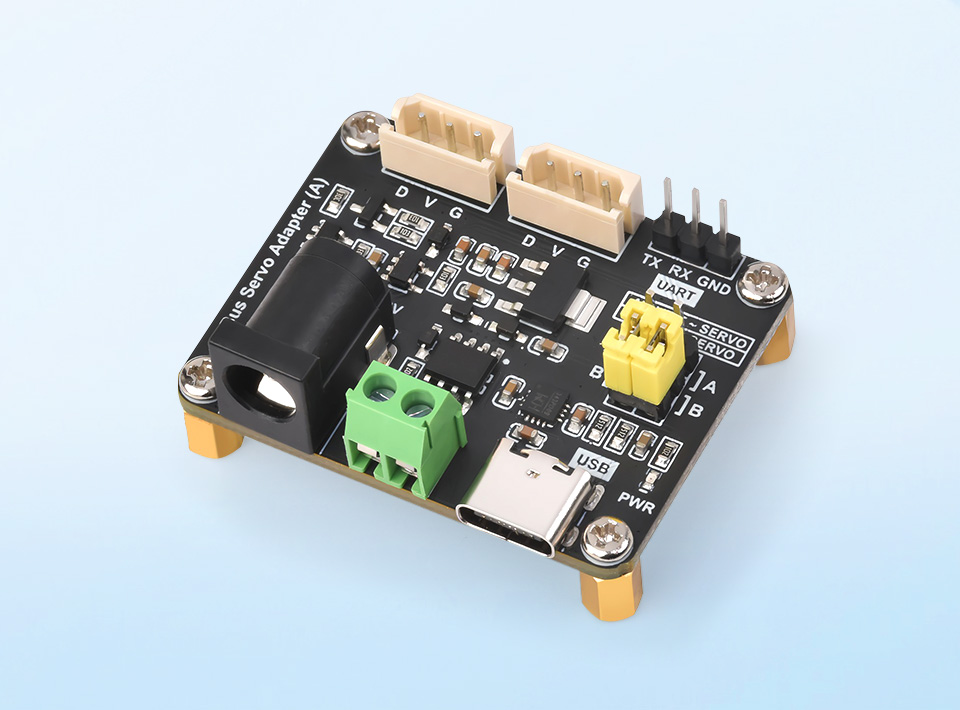
\includegraphics[width=0.6\textwidth]{img/fig36-Bus-Servo-Adapter-A-details-1.jpg} 
    \caption{Bus Servo Adapter (A)}
    \label{fig36}
    \vspace{0.2cm}
\end{figure}

\begin{table}[H]
    \centering
    \caption{Thông số kỹ thuật mạch Bus Servo Adapter (A)}
    \label{tab:adapter_specs}
    \renewcommand{\arraystretch}{1.5} % Tăng độ rộng giữa các hàng cho thoáng và đẹp giống ảnh
    \begin{tabular}{ll}
        \hline
        \textbf{Power Supply} & DC 9 $\sim$ 12.6V (ST series servo) \\ \hline
        \textbf{Power supply connector} & 5.5 $\times$ 2.1mm DC \\ \hline
        \textbf{communication interface} & UART \\ \hline
        \textbf{Dimensions} & 42.00 $\times$ 33.00mm \\ \hline
        \textbf{Mounting hole size} & 2.50mm \\ \hline
        \textbf{Mounting hole spacing} & 37.00 $\times$ 28.00mm \\ \hline
    \end{tabular}
\end{table}

\subsection{Bộ đo lường quán tính }

Module IMU (Inertial Measurement Unit) đóng vai trò cốt lõi trong hệ thống phản hồi thăng bằng của robot. Thay vì sử dụng các cảm biến quán tính thô, đồ án này ứng dụng module GY-BNO055 \cite{bno055} --- một board mạch breakout nhỏ gọn được thiết kế trên nền tảng chip cảm biến BNO055 của Bosch Sensortec. Module tích hợp sẵn gia tốc kế 3 trục, con quay hồi chuyển 3 trục, từ kế 3 trục và đặc biệt là một vi xử lý ARM Cortex-M0+ 32-bit chạy thuật toán kết hợp cảm biến (Sensor Fusion) độc quyền của Bosch, cho phép xuất trực tiếp dữ liệu định hướng tuyệt đối mà không cần bộ lọc ngoại vi.

\begin{figure}[H]
\centering

\includegraphics[width=0.55\textwidth]{img/fig37-IMU-BNO055.png}
\caption{Module cảm biến 9 trục thông minh GY-BNO055 (mặt trước và mặt sau)}
\label{fig37}
\vspace{0.2cm}
\end{figure}

Module GY-BNO055 sở hữu kích thước cực kỳ nhỏ gọn (20,9~mm $\times$ 11,9~mm), rất phù hợp để gắn trực tiếp lên khung thân robot mà không chiếm nhiều không gian. Board mạch được bố trí 8 chân tín hiệu gồm: VIN (nguồn cấp), GND (mass), SCL/Rx (xung nhịp I2C hoặc nhận UART), SDA/Tx (dữ liệu I2C hoặc phát UART), ADD (chọn địa chỉ I2C), INT (ngắt ngoài), BOOT (chế độ nạp firmware) và RESET (khởi động lại phần cứng). Mạch tích hợp sẵn bộ ổn áp nội cho phép cấp nguồn linh hoạt từ 3,3V đến 5V qua chân VIN.

Về mặt kiến trúc phần cứng, nhóm đã tối ưu hóa hệ thống bằng cách loại bỏ hoàn toàn vi điều khiển trung gian như cấu trúc dùng STM32. Nền tảng phát triển giờ đây được triển khai trực tiếp trên môi trường hệ điều hành Linux của Jetson Nano. Cảm biến BNO055 được kết nối và giao tiếp thẳng với Jetson Nano thông qua bus I2C (sử dụng hai chân SCL và SDA). Việc lập trình thu thập dữ liệu được thực hiện bằng ngôn ngữ Python. Sự thay đổi này không chỉ giúp giảm thiểu đáng kể độ trễ truyền dữ liệu mà còn tối giản hóa độ phức tạp của việc đi dây phần cứng.

Khác với các cảm biến truyền thống (như MPU6050) dễ bị nhiễu từ môi trường và đòi hỏi người lập trình phải tự xây dựng các bộ lọc toán học phức tạp (như Complementary Filter hay Kalman Filter) trên máy tính chủ, BNO055 xử lý toàn bộ khối lượng công việc này ở cấp độ phần cứng nội bộ. Tính năng Sensor Fusion của BNO055 tự động tính toán và xuất trực tiếp dữ liệu định hướng dưới dạng các góc Euler (Roll, Pitch, Yaw) hoặc Quaternion với độ chính xác cao và tần số cập nhật nhanh. Do đó, bài toán của nhóm được chuyển từ việc ``viết bộ lọc nhiễu'' sang việc quản lý quy trình tự hiệu chuẩn của cảm biến.
\begin{table}[H]
\centering
\caption{Thông số kỹ thuật module cảm biến GY-BNO055}
\label{tab:bno055_specs}
\renewcommand{\arraystretch}{1.3}
\begin{tabular}{ll}
\toprule
\textbf{Thông số} & \textbf{Giá trị} \\
\midrule
Chip cảm biến & Bosch BNO055 (SiP -- System in Package) \\
Số trục đo & 9 trục (Accelerometer + Gyroscope + Magnetometer) \\
Điện áp hoạt động & 3.3V -- 5V (qua chân VIN, tích hợp bộ ổn áp nội) \\
Chuẩn giao tiếp & I2C / UART (chọn qua chân BOOT) \\
Địa chỉ I2C mặc định & 0x28 (chân ADD = LOW); 0x29 (chân ADD = HIGH) \\
Gia tốc kế (Accelerometer) & $\pm$2g / $\pm$4g / $\pm$8g / $\pm$16g \\
Con quay hồi chuyển (Gyroscope) & $\pm$125$^\circ$/s đến $\pm$2000$^\circ$/s \\
Từ kế (Magnetometer) & $\pm$1300$\mu$T (trục x,y); $\pm$2500$\mu$T (trục z) \\
Bộ xử lý tích hợp & ARM Cortex-M0+ (chạy thuật toán Sensor Fusion) \\
Dữ liệu đầu ra & Quaternion, góc Euler, vector trọng lực, gia tốc tuyến tính \\
Tần số cập nhật Fusion & Lên đến 100 Hz \\
Kích thước mạch & 20,9 $\times$ 11,9 mm \\
Số chân tín hiệu & 8 (VIN, GND, SCL/Rx, SDA/Tx, ADD, INT, BOOT, RESET) \\
Nhiệt độ hoạt động & $-40^\circ$C đến $+85^\circ$C \\
\bottomrule
\end{tabular}
\end{table}
\subsection{Mạch Giảm Áp }

Bên cạnh nguồn năng lượng 12V cung cấp trực tiếp cho hệ thống động cơ servo, thiết bị xử lý trung tâm là máy tính nhúng Jetson Nano Developer Kit B01 yêu cầu một nguồn điện DC 5V ổn định để hoạt động. Trong các điều kiện tải nặng, chẳng hạn như khi tính toán động học nghịch liên tục cho 12 bậc tự do hoặc xử lý thuật toán cân bằng, Jetson Nano có thể tiêu thụ dòng điện lên đến 4A. Việc sử dụng các IC ổn áp tuyến tính thông thường sẽ gây ra hiện tượng hao phí nhiệt lượng rất lớn và không đáp ứng đủ dòng tải yêu cầu.

Do đó, mạch giảm áp xung\textbf{XL4015 5A 75W} đã được lựa chọn để thực hiện nhiệm vụ chuyển đổi điện áp từ 12V của nguồn tổ ong xuống mức 5V an toàn cho Jetson Nano. Ưu điểm nổi bật của XL4015 là hiệu suất chuyển đổi năng lượng cao (lên đến 96\%), tần số băm xung 180KHz giúp giảm thiểu gợn điện áp, và khả năng cấp dòng đầu ra tối đa lên tới 5A. Điều này tạo ra một biên độ dự trữ công suất an toàn, giúp máy tính nhúng không bị sụt áp đột ngột dẫn đến tắt nguồn trong quá trình vận hành. Hơn nữa, mạch còn được tích hợp các tính năng bảo vệ ngắn mạch và bảo vệ quá nhiệt, đảm bảo an toàn tối đa cho các bo mạch điện tử đắt tiền phía sau.

\begin{figure}[H]
    \centering
    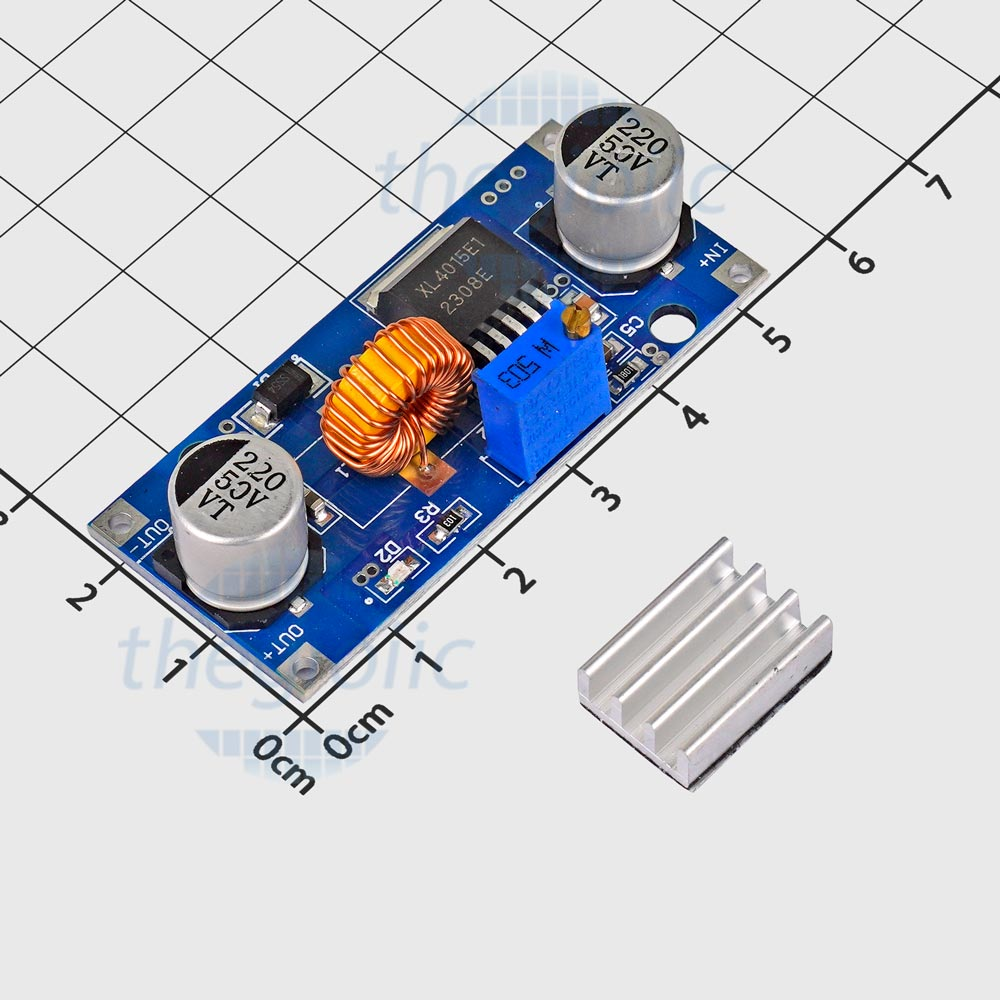
\includegraphics[width=0.6\textwidth]{img/fig38-Mạch giảm áp.jpg} 
    \caption{Mạch giảm áp XL4015 5A 75W}
    \label{fig38}
    \vspace{0.2cm}
\end{figure}

Các thông số kỹ thuật chi tiết của mạch giảm áp XL4015 được trình bày cụ thể trong Bảng \ref{tab:xl4015_specs}. Mức điện áp ngõ ra đã được nhóm tác giả tinh chỉnh qua biến trở tích hợp trên mạch để đạt chính xác mức 5.0V - 5.1V nhằm bù trừ sụt áp trên dây dẫn trước khi cấp vào Jetson Nano.

\begin{table}[H]
    \centering
    \caption{Thông số kỹ thuật mạch giảm áp XL4015 5A 75W}
    \label{tab:xl4015_specs}
    \renewcommand{\arraystretch}{1.5} 
    \begin{tabular}{ll}
        \hline
        \textbf{Điện áp ngõ vào} & 5 $\sim$ 32 VDC \\ \hline
        \textbf{Điện áp ngõ ra} & 1.25 $\sim$ 30 VDC (Tinh chỉnh về 5V cấp cho vi xử lý) \\ \hline
        \textbf{Dòng ngõ ra} & 0 $\sim$ 5A \\ \hline
        \textbf{Công suất ngõ ra} & 75W \\ \hline
        \textbf{Nhiệt độ làm việc} & -40 $\sim$ +85$^\circ$C \\ \hline
        \textbf{Tần số hoạt động} & 180KHz \\ \hline
        \textbf{Hiệu suất tối đa} & 96\% \\ \hline
        \textbf{Bảo vệ ngắn mạch} & Có (giới hạn 8A) \\ \hline
        \textbf{Bảo vệ quá nhiệt} & Có \\ \hline
    \end{tabular}
\end{table}


\subsection{Cơ cấu chấp hành: Động cơ Bus Servo ST3215}

Việc lựa chọn cơ cấu chấp hành có ảnh hưởng trực tiếp đến hiệu năng di chuyển, khả năng giữ thăng bằng và độ phức tạp của hệ thống phần cứng robot bốn chân. Trong đồ án này, động cơ Bus Servo ST3215 và phiên bản tốc độ cao ST3215-HS \cite{waveshare_st3215} đã được lựa chọn làm thiết bị truyền động cho toàn bộ 12 bậc tự do của robot. 

Để làm rõ tính ưu việt và lý do lựa chọn công nghệ truyền động này cho mô hình nguyên mẫu, nhóm đã tiến hành đánh giá và so sánh dòng động cơ Bus Servo nối tiếp với hai loại cơ cấu chấp hành phổ biến khác: Động cơ Servo điều khiển bằng xung PWM truyền thống và Động cơ không chổi than (BLDC).

\begin{table}[H]
\centering
\caption{Bảng so sánh các loại cơ cấu chấp hành áp dụng cho Robot bốn chân}
\label{tab:motor_comparison}
\renewcommand{\arraystretch}{1.3}
\begin{tabular}{|p{0.2\linewidth}|p{0.2\linewidth}|p{0.2\linewidth}|p{0.25\linewidth}|}
\hline
\textbf{Tiêu chí} & \textbf{Động cơ Servo PWM truyền thống} & \textbf{Động cơ BLDC (Tích hợp Driver)} & \textbf{Động cơ Bus Servo nối tiếp} \\ \hline
\textbf{Giao thức điều khiển} & Xung PWM (Đơn hướng) & CAN / RS485 (Song công) & UART bán song công (Half-duplex) \\ \hline
\textbf{Hệ thống dây dẫn} & Rất phức tạp (Mỗi motor 1 dây tín hiệu riêng) & Tối giản (Nối tiếp chuỗi - Daisy chain) & Tối giản (Nối tiếp chuỗi - Daisy chain) \\ \hline
\textbf{Khả năng phản hồi (Feedback)} & Không có & Vị trí, tốc độ, dòng điện, nhiệt độ (FOC) & Vị trí thực tế, tốc độ, tải, nhiệt độ, điện áp \\ \hline
\textbf{Mô-men xoắn} & Thường ở mức thấp đến trung bình & Rất cao & Cao (Tối ưu trong tầm giá) \\ \hline
\textbf{Khối lượng \& Kích thước} & Nhẹ & Nặng, cồng kềnh & Gọn nhẹ \\ \hline
\textbf{Giá thành} & Rất thấp & Rất cao & Trung bình - Hợp lý \\ \hline
\textbf{Độ phù hợp} & Thấp (Do không có phản hồi và thiếu lực) & Thấp (Dư thừa công suất, chi phí quá cao) & \textbf{Rất cao (Đạt điểm cân bằng tối ưu)} \\ \hline
\end{tabular}
\end{table}

Sau khi xác định kiến trúc truyền động tối ưu là sử dụng \textbf{Bus Servo nối tiếp} thay vì Servo PWM hay động cơ BLDC, nhóm đã tiến hành khảo sát và đánh giá các dòng Bus Servo phổ biến trên thị trường để tìm ra phương án phù hợp nhất cho hệ thống 12 bậc tự do của robot.

Ba đại diện tiêu biểu được đưa ra so sánh bao gồm: Hiwonder LX-16A, Waveshare ST3215 và Dynamixel XL430-W250-T.

\begin{table}[H]
\centering
\caption{So sánh các dòng Bus Servo nối tiếp phổ biến trên thị trường}
\label{tab:bus_servo_comparison}
\renewcommand{\arraystretch}{1.3}
\begin{tabular}{|p{0.2\linewidth}|p{0.2\linewidth}|p{0.25\linewidth}|p{0.2\linewidth}|}
\hline
\textbf{Tiêu chí} & \textbf{Hiwonder LX-16A} & \textbf{Waveshare ST3215 (Được chọn)} & \textbf{Dynamixel XL430-W250-T} \\ \hline
\textbf{Giao thức} & TTL UART (Half-duplex) & TTL UART (Half-duplex) & TTL UART (Half-duplex) \\ \hline
\textbf{Điện áp} & 6.0V - 8.4V (Tối ưu 7.4V) & 6.0V - 12.6V (Tối ưu 12V) & 10.0V - 14.8V (Tối ưu 11.1V) \\ \hline
\textbf{Lực xoắn tối đa} & 17 kg.cm (@7.4V) & 30 kg.cm / 20 kg.cm (@12V) & $\sim$15.3 kg.cm (1.5 N.m @11.1V) \\ \hline
\textbf{Cảm biến vị trí} & Biến trở (Potentiometer) & Từ tính (Magnetic Encoder $360^{\circ}$) & Từ tính (Absolute Encoder) \\ \hline
\textbf{Độ phân giải góc} & 0.24$^{\circ}$ & 0.088$^{\circ}$ & 0.088$^{\circ}$ \\ \hline
\textbf{Tốc độ truyền} & 115200 bps & Lên đến 1 Mbps & Lên đến 4.5 Mbps \\ \hline
\textbf{Bộ điều khiển} & Cơ bản (P) & Nâng cao (PI) & Cao cấp (PID vị trí, vận tốc, dòng) \\ \hline
\textbf{Giá thành} & Thấp ($\sim$300.000 VNĐ) & Trung bình ($\sim$500.000 VNĐ) & Rất cao ($\sim$1.500.000 VNĐ) \\ \hline
\end{tabular}
\end{table}

Dựa trên các thông số phân tích từ Bảng \ref{tab:bus_servo_comparison}, Waveshare ST3215 được lựa chọn là giải pháp tối ưu nhất cho hệ thống cơ cấu chấp hành của đồ án vì những lý do sau:

\begin{itemize}
    \item \textbf{Khắc phục nhược điểm của LX-16A:} Mặc dù Hiwonder LX-16A có lợi thế về giá thành thấp, nhưng lực xoắn tối đa chỉ đạt 17 kg.cm, không đủ để đáp ứng tải trọng động khi robot di chuyển hoặc thực hiện các tư thế phức tạp. Hơn nữa, việc sử dụng biến trở (Potentiometer) làm cảm biến vị trí khiến độ phân giải góc thấp ($0.24^{\circ}$) và dễ bị hao mòn cơ học theo thời gian. Bộ điều khiển của LX-16A chỉ dừng ở mức cơ bản (P), dẫn đến sai số tĩnh lớn và khả năng bám quỹ đạo kém.
    \item \textbf{Cân bằng hiệu năng và chi phí so với Dynamixel:} Dòng Dynamixel XL430-W250-T sở hữu bộ điều khiển PID hoàn chỉnh cùng nhiều tính năng cao cấp. Tuy nhiên, mức giá cực kỳ đắt đỏ (gấp khoảng 3 lần ST3215). Với yêu cầu 12 bậc tự do, việc sử dụng Dynamixel sẽ làm chi phí phần cứng vượt quá ngân sách cho phép. Thêm vào đó, lực xoắn của XL430-W250-T ($\sim$15.3 kg.cm) lại thấp hơn ST3215, đòi hỏi phải sử dụng cơ cấu truyền động phức tạp để khuyếch đại lực.
    \item \textbf{Ưu điểm vượt trội của ST3215:} Waveshare ST3215 mang lại điểm cân bằng hoàn hảo giữa hiệu năng cơ học và chi phí. Lực xoắn cao (lên đến 30 kg.cm ở 12V) cung cấp dư dả công suất để robot duy trì thăng bằng và thực hiện dáng đi. Cảm biến vị trí từ tính (Magnetic Encoder $360^{\circ}$) với độ phân giải rất cao ($0.088^{\circ}$) cung cấp phản hồi góc chính xác tuyệt đối mà không lo bị hao mòn. Tốc độ truyền tải 1 Mbps hoàn toàn đáp ứng được yêu cầu của vòng lặp điều khiển thời gian thực. Đặc biệt, bộ điều khiển PI tích hợp sẵn giúp động cơ khử sai số tĩnh, đảm bảo robot bám sát quỹ đạo dáng đi một cách mượt mà và ổn định.
\end{itemize}

\subsection{Hệ thống Phân phối Năng lượng và Lựa chọn Dây dẫn}

Để đảm bảo hệ thống 12 động cơ hoạt động ổn định ở dòng tải cao mà không bị sụt áp, việc thiết kế sơ đồ đi dây và lựa chọn tiết diện dây dẫn đóng vai trò cực kỳ quan trọng. Dựa trên phân tích dòng điện tổng ($I_{total} \approx 32.4A$) từ nguồn tổ ong, hệ thống dây dẫn được chia thành 3 cấp độ với các tiêu chuẩn AWG (American Wire Gauge) khác nhau, được phân phối qua các khối đầu nối nguồn (Terminal Block).

\begin{figure}[H]
    \centering
    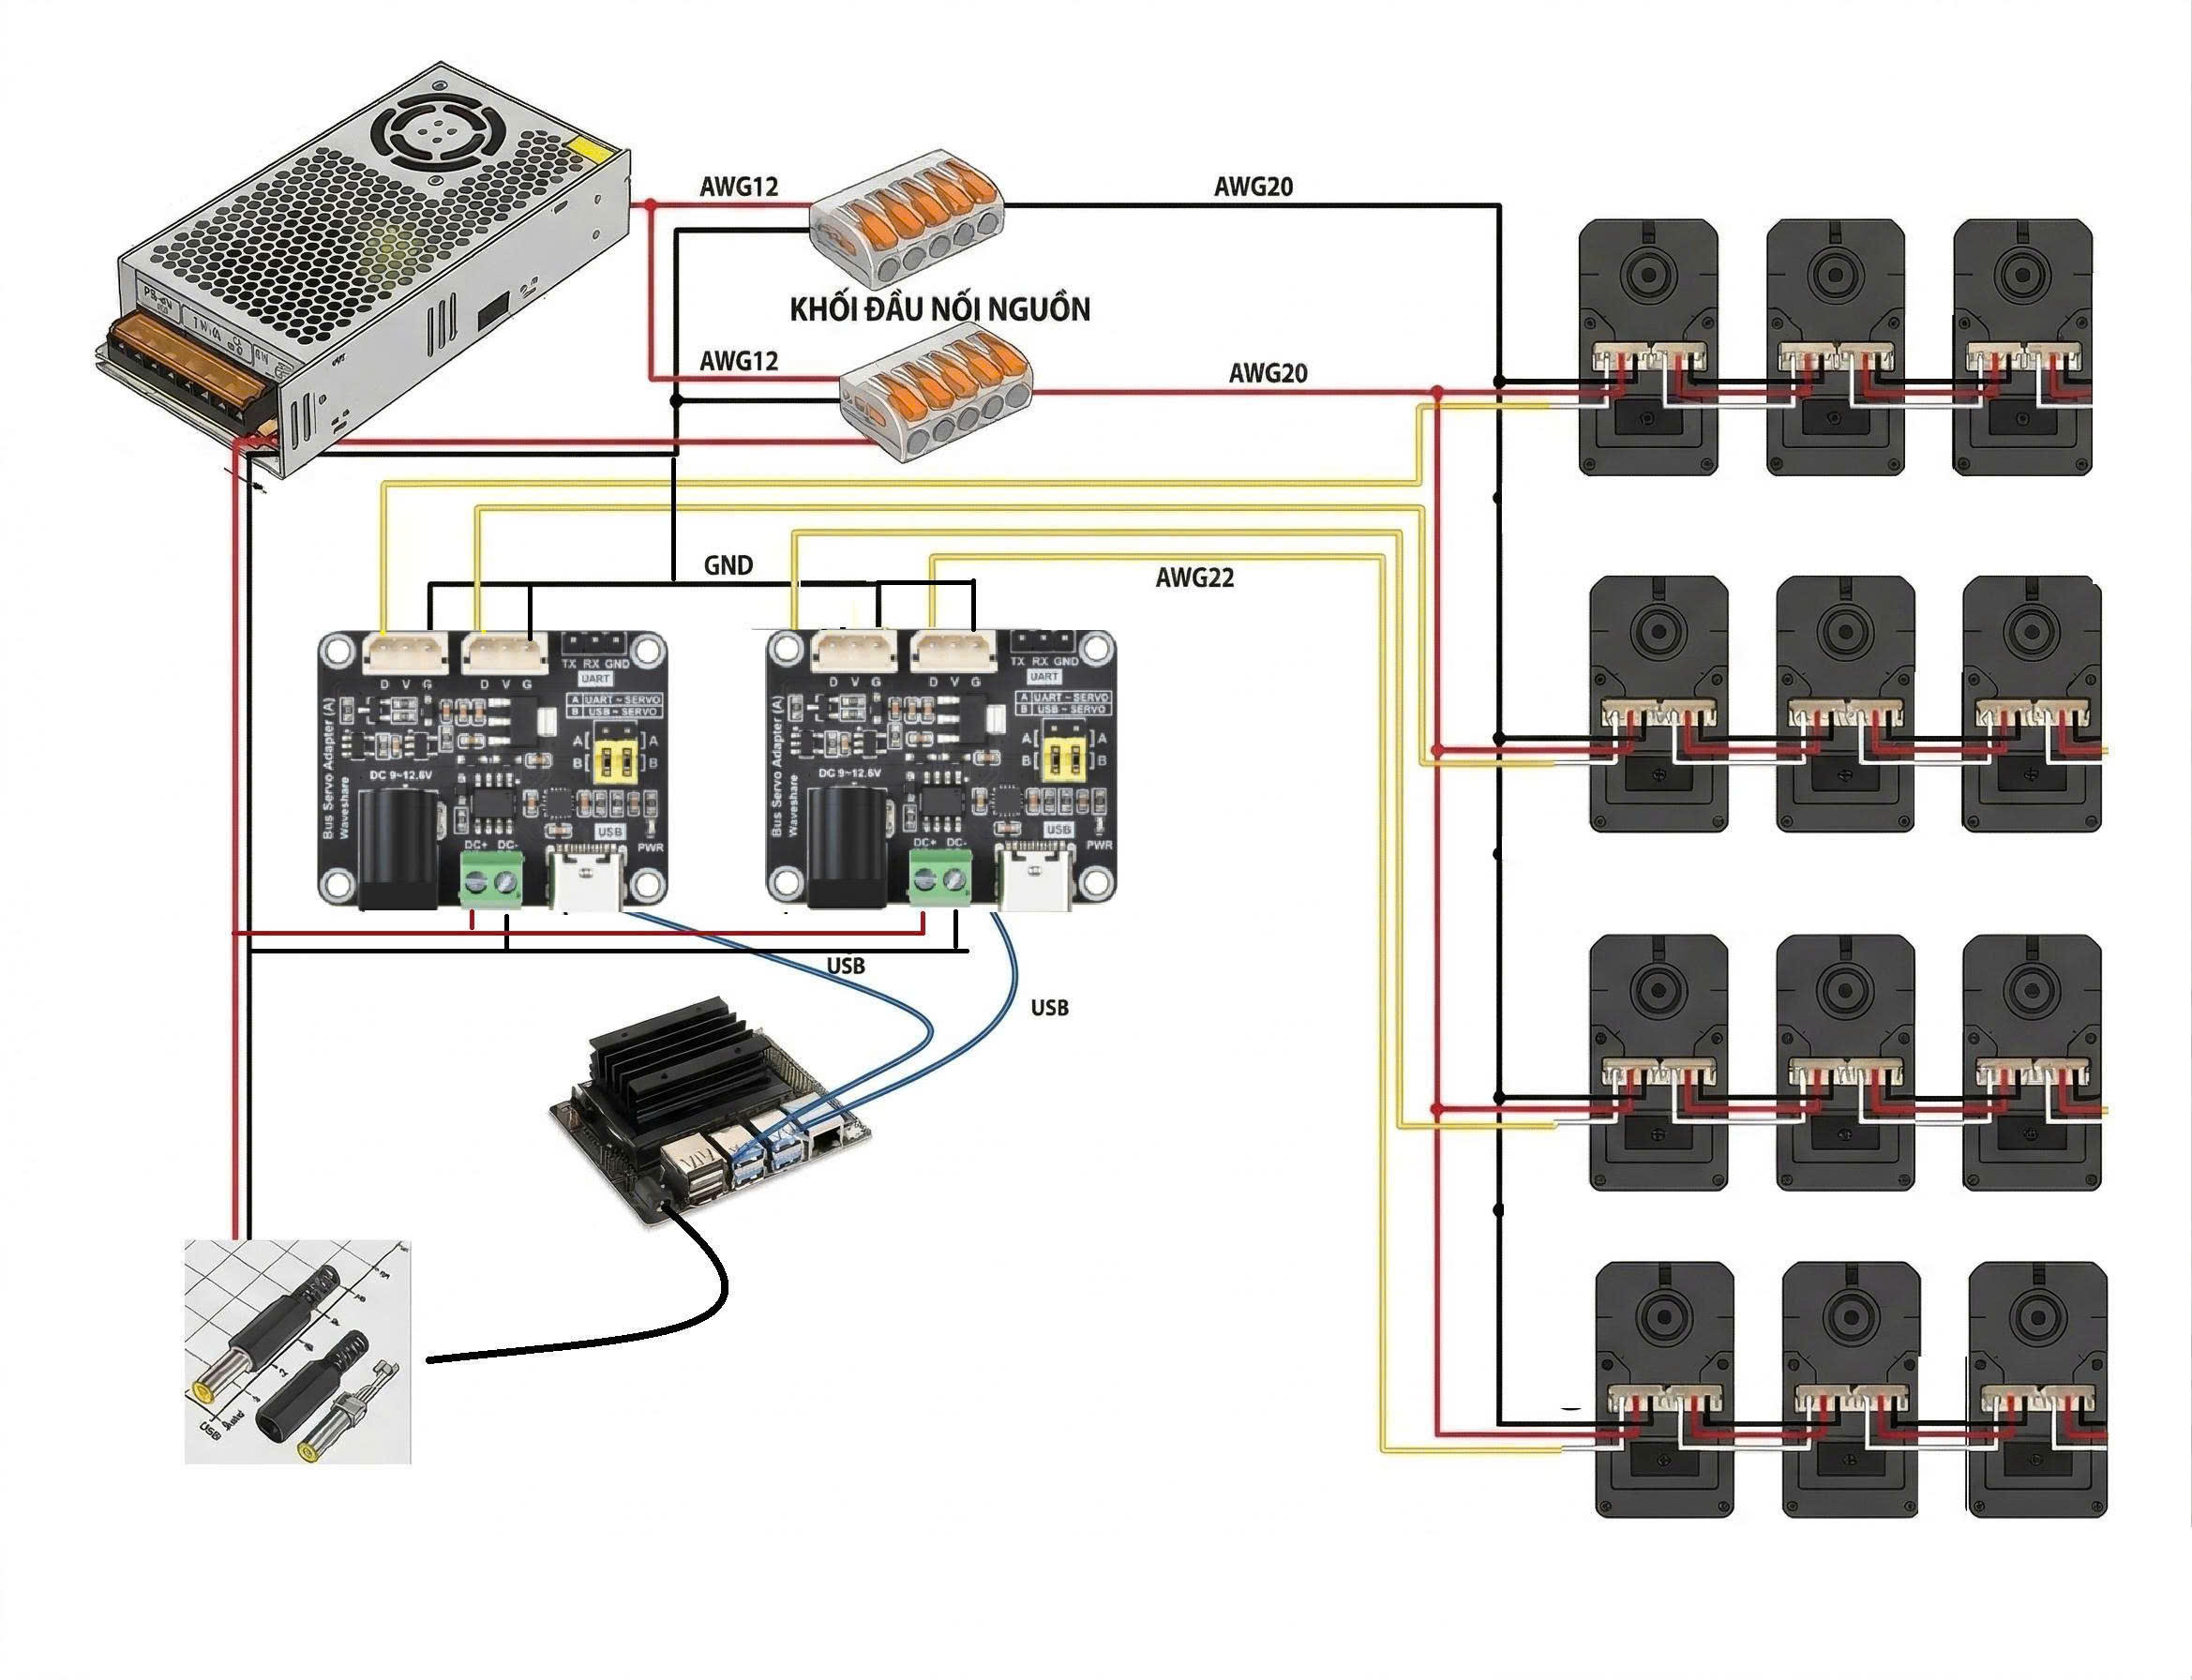
\includegraphics[width=1.0\textwidth]{img/fig44-sododiday-hethong.jpg} 
    \caption{Sơ đồ phân phối điện áp và tín hiệu tổng thể của robot}
    \label{fig44}
    \vspace{0.2cm}
\end{figure}

Dựa trên thông số kỹ thuật (Datasheet) của các loại dây lõi đồng, nhóm đã đưa ra thiết kế đi dây như sau:

\textbf{1. Trục nguồn chính (Từ Nguồn tổ ong đến Khối đấu nối): Dây AWG 12}
\begin{itemize}
    \item \textbf{Chức năng:} Truyền tải toàn bộ dòng điện từ nguồn xung 12V-40A đến các khối chia nguồn trung tâm.
    \item \textbf{Thông số kỹ thuật (AWG 12):} Đường kính lõi khoảng 2.05 mm, tiết diện 3.31 mm$^2$. Khả năng chịu dòng (Ampacity) trong điều kiện không khí mở có thể lên đến 30A - 40A, với điện trở cực kỳ thấp (khoảng 5.2 $\Omega$/km).
    \item \textbf{Lý do lựa chọn:} Trục chính phải gánh toàn bộ tải của 12 servo cùng lúc (dòng xả tức thời có thể đạt 32.4A). Dây AWG 12 hoàn toàn đáp ứng được mức dòng điện này mà không sinh nhiệt hay gây sụt áp đáng kể trên đường truyền.
\end{itemize}

\textbf{2. Nhánh nguồn phụ (Từ Khối đấu nối đến Servo đầu tiên): Dây AWG 20}
\begin{itemize}
    \item \textbf{Chức năng:} Cấp nguồn trực tiếp từ khối chia nguồn đến động cơ Servo đầu tiên của mỗi nhánh (chuỗi 3 servo cho mỗi chân).
    \item \textbf{Thông số kỹ thuật (AWG 20):} Đường kính lõi 0.81 mm, tiết diện 0.52 mm$^2$. Khả năng chịu dòng định mức khoảng 5A (tối đa có thể lên 11A tùy lớp cách điện).
    \item \textbf{Lý do lựa chọn:} Mỗi nhánh chân gồm 3 servo ST3215, với dòng khởi động tổng cộng khoảng 8.1A. Dây AWG 20 cung cấp sự cân bằng hoàn hảo giữa khả năng chịu tải và độ linh hoạt (mềm dẻo) để luồn lách qua các khớp cơ khí của robot.
\end{itemize}

\textbf{3. Bus tín hiệu truyền thông (Từ Adapter đến Servo): Dây AWG 22}
\begin{itemize}
    \item \textbf{Chức năng:} Truyền tín hiệu UART (Data) từ mạch Bus Servo Adapter đến các servo, và kết nối chung chân Mass (GND) để đồng bộ mức điện áp logic.
    \item \textbf{Thông số kỹ thuật (AWG 22):} Đường kính lõi 0.64 mm, tiết diện 0.326 mm$^2$. 
    \item \textbf{Lý do lựa chọn:} Đường truyền dữ liệu không mang dòng điện tải cao (chỉ vài mA). Việc sử dụng dây AWG 22 giúp cáp tín hiệu nhỏ gọn, hạn chế nhiễu chéo, dễ dàng bấm cos và đi dây nối tiếp (daisy-chain) qua từng servo mà không gây cản trở chuyển động của các khớp.
\end{itemize}

Việc thiết kế phân nhánh nguồn thông qua Terminal Block kết hợp với việc tính toán và lựa chọn đúng cỡ dây AWG từ datasheet giúp giải quyết triệt để vấn đề sụt áp trên đường dây (Voltage Drop), đảm bảo 12 động cơ ở cuối chuỗi vẫn nhận đủ điện áp 12V để sinh ra mô-men xoắn tối đa.

\section{Các Giao thức Truyền thông của Hệ thống}

Toàn bộ hệ thống điều khiển sử dụng hai giao thức truyền thông chính: I2C để thu thập dữ liệu cảm biến và UART để điều khiển cơ cấu chấp hành. Vi xử lý trung tâm Jetson Nano đóng vai trò là thiết bị chủ , liên tục nhận dữ liệu tư thế không gian từ module IMU và thực hiện các tính toán động học nghịch dựa trên thông số hình học của các chân. Để hoàn thành nhiệm vụ này, việc đầu tiên nhóm thực hiện là thiết lập giao tiếp I2C giữa Jetson Nano và cảm biến IMU. Đây là một bước có thể thực hiện hiệu quả thông qua môi trường lập trình Python trên hệ điều hành Linux (Ubuntu), bằng cách khai báo đúng địa chỉ phần cứng và sử dụng trực tiếp các chân bus I2C tích hợp sẵn trên bo mạch Jetson.

\begin{figure}[H]
    \centering
    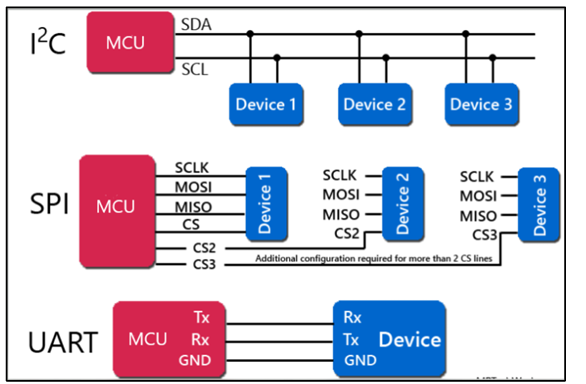
\includegraphics[width=0.6\textwidth]{img/fig39-Different Communication Protocols .png} 
    \caption{Các giao thức truyền thông khác nhau}
    \label{fig39}
    \vspace{0.2cm}
    \textit{}
\end{figure}

Phần công việc đòi hỏi nhiều sự tinh chỉnh và thời gian hoàn thành hơn là việc thiết lập và tối ưu hóa đường truyền tín hiệu xuống các động cơ servo. Để điều khiển đồng bộ 12 động cơ ST3215, hệ thống sử dụng chuẩn giao tiếp UART (thông qua hai cổng USB) kết nối với hai mạch Bus Servo Adapter (A). Các mạch Adapter này hoạt động ở tốc độ truyền tải (baudrate) lên đến 1 Mbps, làm nhiệm vụ phân phối các gói tin lệnh dạng nối tiếp đến từng địa chỉ định danh (ID) của động cơ trên cùng một đường bus truyền tín hiệu tương ứng. Việc chuyển đổi từ tín hiệu mức logic của Jetson Nano sang chuẩn bus nối tiếp bán song công, kết hợp với việc chia thành 2 bus riêng biệt, giúp đơn giản hóa đáng kể sơ đồ đi dây vật lý mà vẫn đảm bảo tốc độ phản hồi siêu tốc độ theo thời gian thực cho vòng lặp điều khiển PID.

\begin{figure}[H]
    \centering
    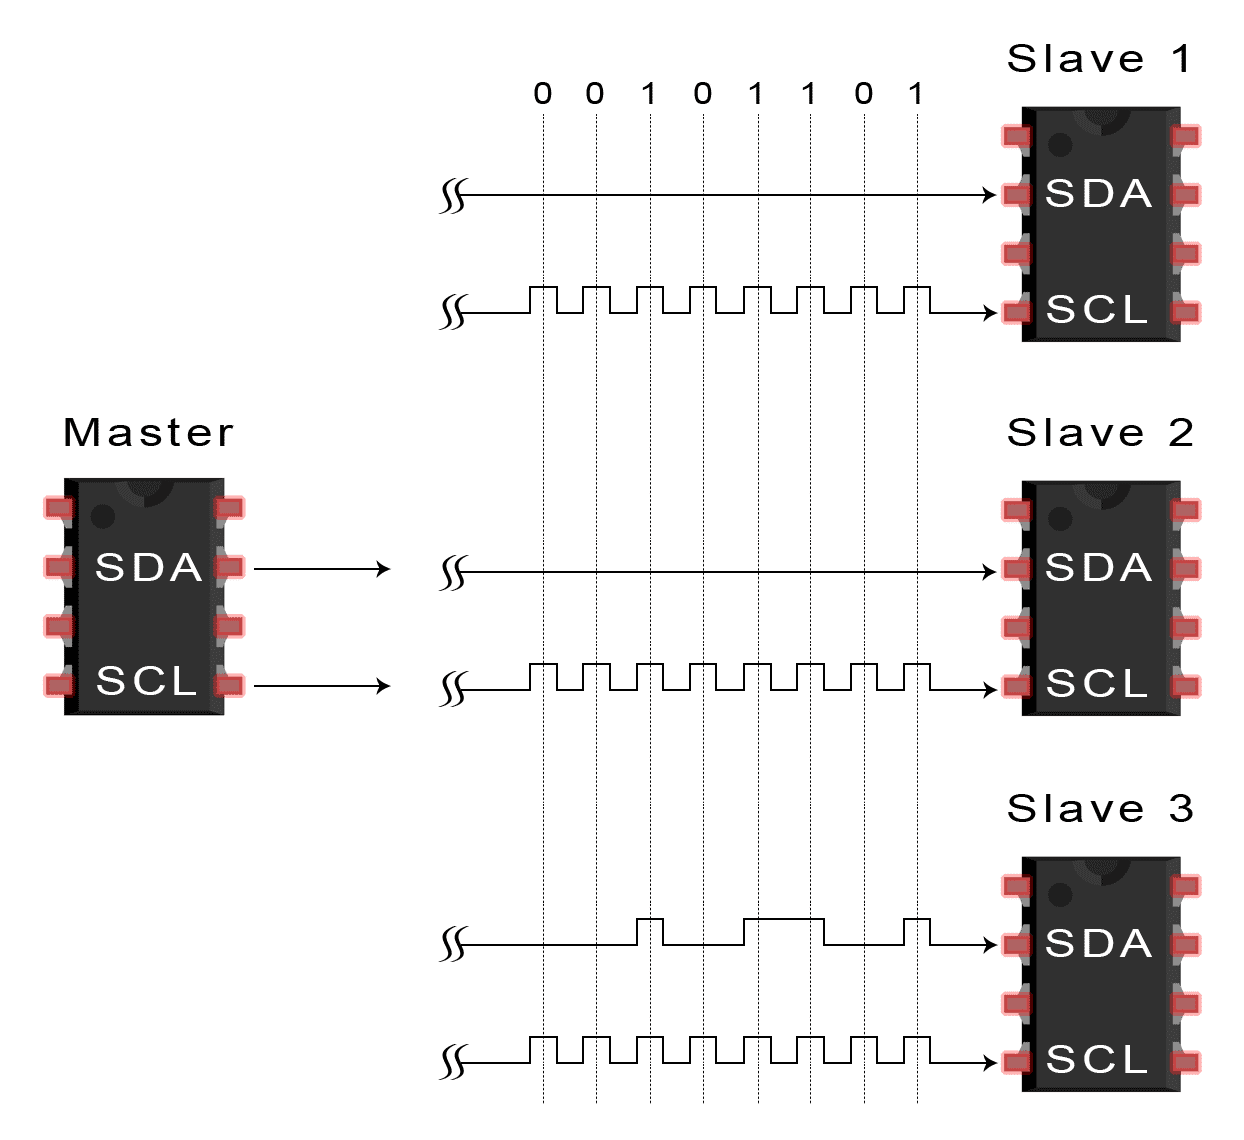
\includegraphics[width=0.6\textwidth]{img/fig40-Introduction-to-I2C-Data-Transmission-Diagram-Data-Frame.png} 
    \caption{Giao thức truyền thông I2C}
    \label{fig40}
    \vspace{0.2cm}
\end{figure}
\begin{figure}[H]
    \centering
    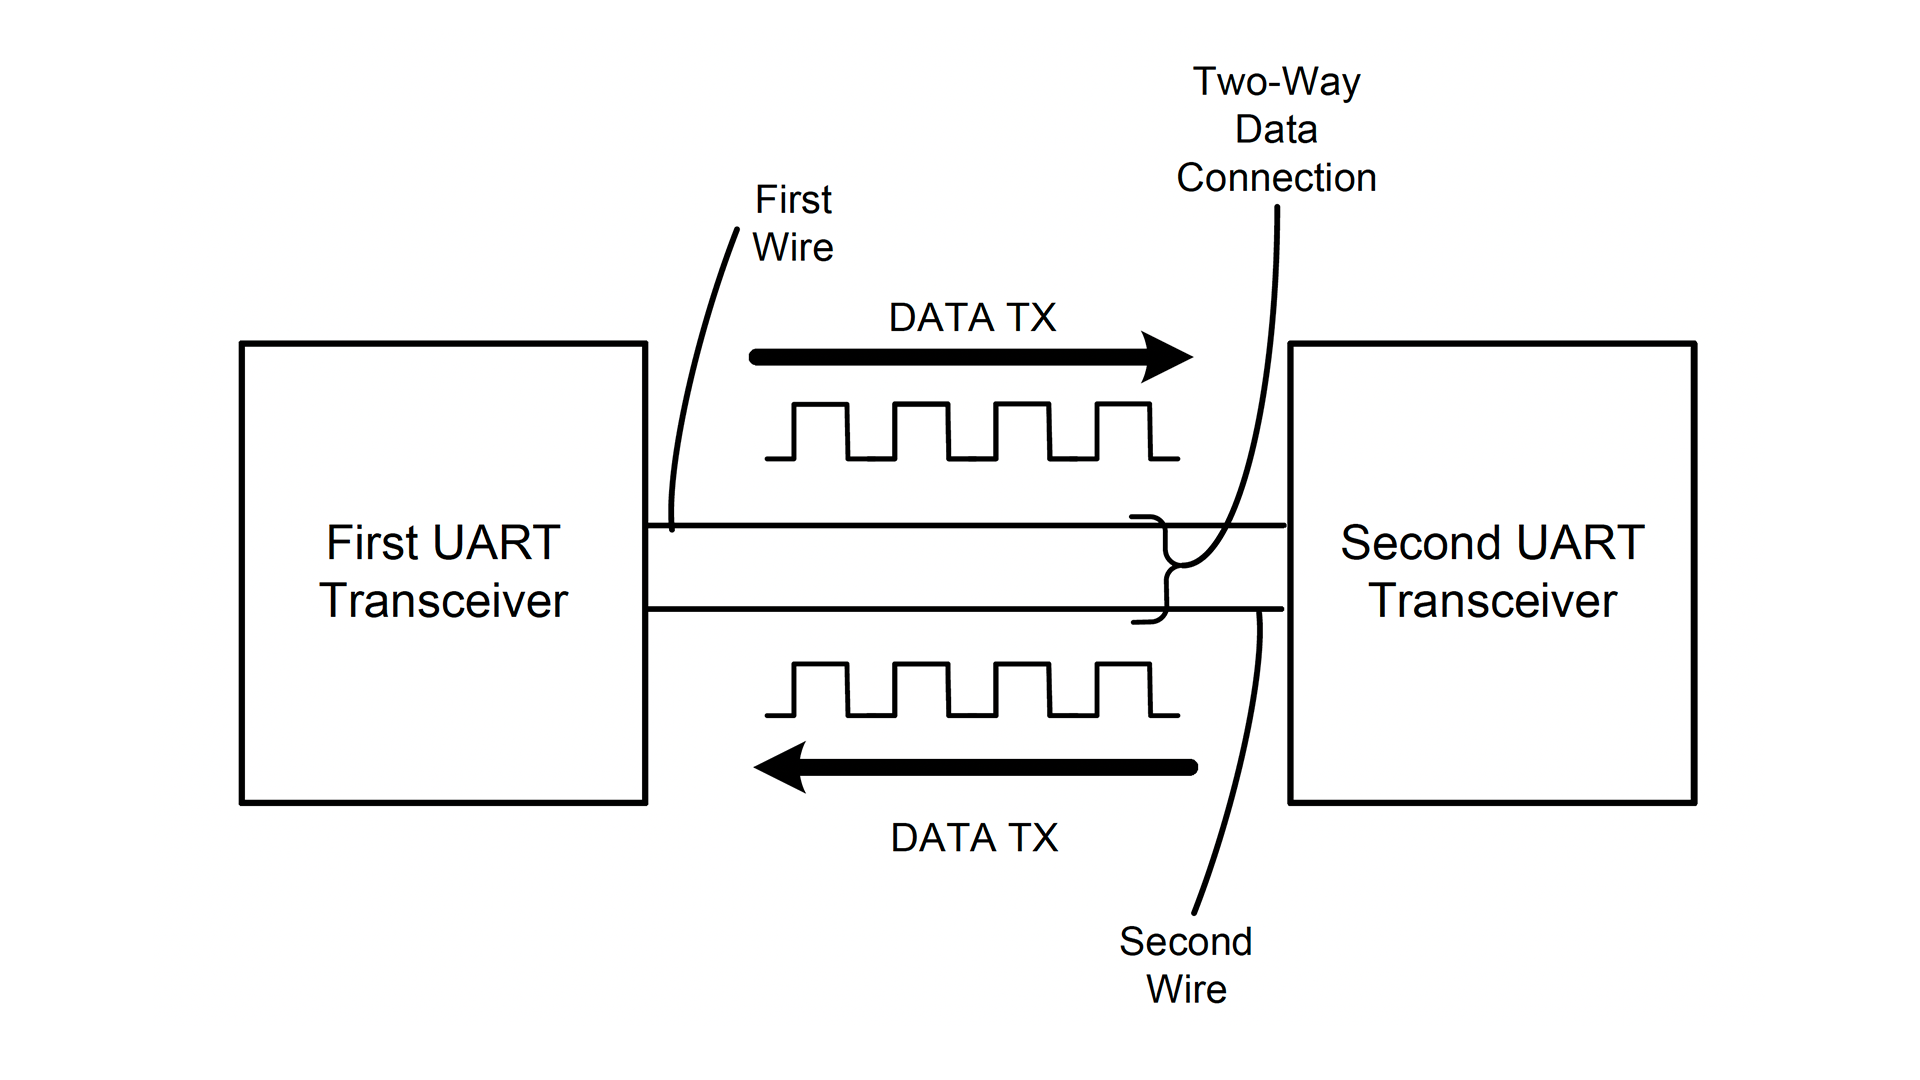
\includegraphics[width=0.6\textwidth]{img/fig41-Wired-UART.png} 
    \caption{Giao thức truyền thông UART}
    \label{fig41}
    \vspace{0.2cm}
\end{figure}

\subsection{Phân tích thời gian truyền thông UART}

Việc phân tích thời gian truyền thông trên bus UART là cần thiết để đảm bảo tốc độ cập nhật lệnh servo đáp ứng yêu cầu thời gian thực của vòng lặp điều khiển. Với baudrate 1 Mbps và giao thức bán song công (half-duplex), mỗi giao dịch bao gồm:

\begin{itemize}
    \item \textbf{Gói lệnh ghi (Write):} Gồm header (2 byte), ID servo (1 byte), chiều dài (1 byte), lệnh (1 byte), dữ liệu vị trí + tốc độ (4 byte), và checksum (1 byte). Tổng: 10 byte.
    \item \textbf{Gói phản hồi (Response):} Gồm header (2 byte), ID (1 byte), chiều dài (1 byte), lỗi (1 byte), dữ liệu (2 byte), và checksum (1 byte). Tổng: 8 byte.
\end{itemize}

Với cấu hình 8N1 (8 bit dữ liệu, không parity, 1 stop bit), mỗi byte cần 10 bit truyền. Thời gian cho một giao dịch hoàn chỉnh (ghi + đọc) với một servo:

\begin{equation}
    t_{servo} = \frac{(10 + 8) \times 10}{10^6} = 180 \; \mu\text{s}
\end{equation}

Mỗi bus driver quản lý 6 servo, thời gian tổng cho một frame lệnh:

\begin{equation}
    t_{bus} = 6 \times t_{servo} = 6 \times 180 = 1080 \; \mu\text{s} \approx 1{,}1 \text{ ms}
\end{equation}

Hai bus hoạt động song song trên hai cổng USB riêng biệt, nên tổng thời gian truyền thông cho 12 servo vẫn xấp xỉ $1{,}1$ ms --- nhỏ hơn nhiều so với chu kỳ điều khiển $\Delta T = 7$ ms. Điều này xác nhận băng thông truyền thông đủ cho vận hành thời gian thực.

\subsection{Ánh xạ ID servo và phân bổ driver}

Bảng~\ref{tab:servo_mapping} trình bày cấu hình ánh xạ ID servo và phân bổ cho hai driver UART.

\begin{table}[H]
\centering
\caption{Ánh xạ ID servo theo driver và chân robot}
\label{tab:servo_mapping}
\renewcommand{\arraystretch}{1.3}
\begin{tabular}{|l|c|c|c|c|}
\hline
\textbf{Chân} & \textbf{Driver} & \textbf{Hip Roll} & \textbf{Hip Pitch} & \textbf{Knee} \\ \hline
Left-Front (LF) & A & ID 7 & ID 8 & ID 9 \\ \hline
Right-Behind (RB) & A & ID 10 & ID 11 & ID 12 \\ \hline
Right-Front (RF) & B & ID 1 & ID 2 & ID 3 \\ \hline
Left-Behind (LB) & B & ID 4 & ID 5 & ID 6 \\ \hline
\end{tabular}
\end{table}

Chiến lược phân bổ ghép hai chân \textit{chéo nhau} trên cùng một driver (LF+RB trên Driver A, RF+LB trên Driver B) có ý nghĩa quan trọng: trong dáng đi Trot, hai chân chéo luôn ở cùng pha (swing hoặc stance). Khi một cặp chéo đang ở pha swing (cần cập nhật vị trí nhanh), cặp còn lại ở pha stance (ít thay đổi), giúp cân bằng tải truyền thông giữa hai bus.

\section{Kiến trúc phần mềm ROS 2}

\subsection{Tổng quan kiến trúc node}

Hệ thống phần mềm được triển khai trên nền tảng ROS~2 Humble \cite{ros2docs}, sử dụng kiến trúc xử lý phân tán gồm hai node tính toán được phân vùng theo chức năng:

\begin{itemize}
    \item \textbf{Gait Generator Node:} Quản lý toàn bộ quá trình tính toán quỹ đạo tuần hoàn, giải bài toán động học nghịch và gửi lệnh điều khiển đến các cơ cấu chấp hành qua bus nối tiếp. Node này được lập trình bằng Python, bao gồm các module: \texttt{gaitGenerator.py} (37KB -- tạo dáng đi), \texttt{kinematics.py} (IK solver), \texttt{quinticPlanning.py} (nội suy đa thức bậc 5) và \texttt{serialPublish.py} (giao tiếp UART với servo).
    
    \item \textbf{Balance Controller Node:} Xử lý bất đồng bộ việc thu thập dữ liệu quán tính tần số cao, xử lý tín hiệu đa giai đoạn và tính toán bù PID. Node này hoạt động độc lập qua module \texttt{nodeBalanceController.py} (22KB).
\end{itemize}

\subsection{Giao tiếp giữa các node}

Giao tiếp liên tiến trình giữa hai node sử dụng cơ chế publish-subscribe qua DDS (Data Distribution Service) của ROS~2. Balance Controller node phát các thông điệp vector hiệu chỉnh nhẹ trên các topic bất đồng bộ chuyên dụng. Kiến trúc tách rời này đảm bảo rằng các nút thắt xử lý tại Gait Generator không thể chiếm quyền hoặc chặn các bù trừ cảm biến quan trọng, cho phép vận hành xác định, chịu lỗi ngay cả dưới tải CPU cao.

Sơ đồ tổng thể kiến trúc ROS~2 bao gồm các node, topic và luồng dữ liệu giữa các thành phần được thể hiện trong Hình~\ref{fig:ros2_arch}. Sơ đồ phân biệt rõ các thành phần theo loại: ROS~2 node (Python), driver (C++), topic truyền thông, cảm biến phần cứng, và giao diện mô phỏng Gazebo.

\begin{figure}[H]
    \centering
    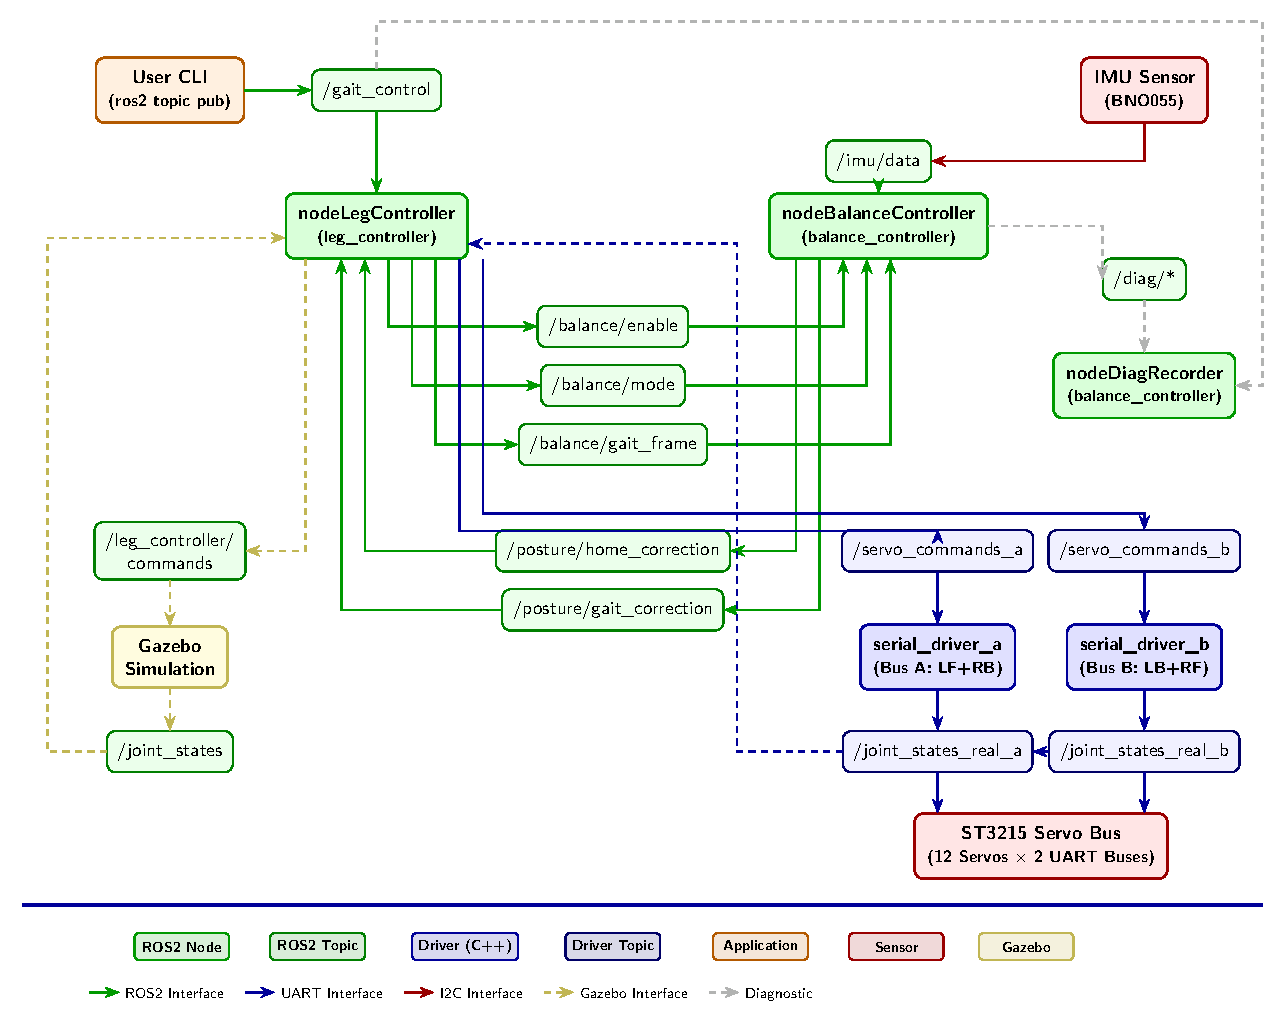
\includegraphics[width=\textwidth]{img/fig_ros2_architecture.pdf}
    \caption{Sơ đồ kiến trúc ROS~2 của hệ thống: các node, topic và luồng dữ liệu}
    \label{fig:ros2_arch}
\end{figure}

\subsection{Các trạng thái vận hành}

Hệ thống quản lý hai trạng thái vận hành rời rạc thông qua cổng logic boolean:

\begin{itemize}
    \item \textbf{HOME:} Cấu hình tĩnh không có vector tịnh tiến tuần hoàn. Bộ điều khiển tính toán các điều chỉnh đồng nhất trong không gian khớp, ánh xạ cứng đến tư thế nghỉ. Sai lệch góc cơ sở được chuyển đổi tỷ lệ thành các bù mô-men đối kháng nhằm hiệu chỉnh tư thế liên tục. Một khoảng trễ khởi động $T_{delay}$ giây có thể cấu hình giúp ngăn hiệu chỉnh sớm trong giai đoạn quá độ khởi tạo hệ thống.
    
    \item \textbf{GAIT:} Trạng thái động kích hoạt khi có lệnh tịnh tiến mặt phẳng. Robot thực hiện quỹ đạo đa thức tuần hoàn sử dụng các mảng dịch pha khả cấu hình để tạo dáng đi trot ($\phi = [0, 0, 0{,}5, 0{,}5]$), walk ($\phi = [0, 0{,}25, 0{,}5, 0{,}75]$) và các dáng đi khác. Các hiệu chỉnh không gian từ phản hồi quán tính chỉ được áp dụng cho chân ở pha chống, trong khi chân ở pha bay duy trì bù bằng không để đảm bảo khoảng trống sải bước.
\end{itemize}

\subsection{Cấu trúc các ROS 2 packages}

Toàn bộ hệ thống phần mềm được tổ chức thành 6 packages ROS~2:

\begin{table}[H]
\centering
\caption{Cấu trúc các ROS 2 packages trong hệ thống}
\label{tab:ros2_packages}
\renewcommand{\arraystretch}{1.3}
\begin{tabular}{|p{0.22\linewidth}|p{0.12\linewidth}|p{0.52\linewidth}|}
\hline
\textbf{Package} & \textbf{Ngôn ngữ} & \textbf{Chức năng} \\ \hline
\texttt{leg\_controller} & Python & Tạo dáng đi, IK solver, quy hoạch quỹ đạo, giao tiếp servo \\ \hline
\texttt{balance\_controller} & Python & Thu thập IMU, xử lý tín hiệu, PID cân bằng, chẩn đoán \\ \hline
\texttt{serial\_driver} & C++ & Driver giao tiếp với bus servo ST3215 (thư viện SCServo) \\ \hline
\texttt{simulation} & Python & Mô hình URDF, cấu hình Gazebo, RViz, launch mô phỏng \\ \hline
\texttt{launch\_main} & CMake & Launch files cho hệ thống thực \\ \hline
\end{tabular}
\end{table}

\subsection{Chi tiết các module phần mềm}

\textbf{Module gaitGenerator.py} là module cốt lõi của hệ thống, quản lý máy trạng thái (state machine) điều khiển toàn bộ vòng đời vận hành của robot. Module này thực hiện các chức năng:

\begin{itemize}
    \item \textbf{Quản lý trạng thái:} Robot chuyển đổi giữa các trạng thái: INIT (khởi tạo) $\rightarrow$ ZERO (homing về tư thế đứng) $\rightarrow$ TROT/WALK/PUSHUP/SWAY (dáng đi) $\rightarrow$ ROBOTOFF (tắt an toàn). Mỗi trạng thái có hàm \texttt{control\_tick()} riêng biệt xử lý một frame điều khiển.
    \item \textbf{Tạo quỹ đạo:} Gọi hàm \texttt{quintic\_planning()} để tạo quỹ đạo hình chữ D cho mỗi chân, sau đó giải IK qua module \texttt{kinematics.py} để chuyển đổi từ tọa độ Đề-các sang góc khớp.
    \item \textbf{Áp dụng hiệu chỉnh IMU:} Nhận tín hiệu bù từ Balance Controller qua hai topic \texttt{/posture/home\_correction} và \texttt{/posture/gait\_correction}, áp dụng vào góc khớp (HOME) hoặc tọa độ bàn chân (GAIT).
    \item \textbf{Xuất lệnh servo:} Gửi góc điều khiển đến module \texttt{serialPublish.py} để chuyển đổi từ góc IK sang góc servo và truyền qua UART.
\end{itemize}

\textbf{Module serialPublish.py} đảm nhận việc chuyển đổi giữa hai chế độ vận hành (mô phỏng và phần cứng thực) thông qua biến cấu hình \texttt{use\_real}:

\begin{itemize}
    \item \textbf{Chế độ mô phỏng:} Xuất bản lệnh mô-men (effort) lên topic \texttt{/effort\_controller/commands} để điều khiển robot trong Gazebo thông qua plugin \texttt{gazebo\_ros2\_control}.
    \item \textbf{Chế độ phần cứng:} Chuyển đổi góc IK sang góc servo bằng các hàm ánh xạ riêng biệt cho từng chân (\texttt{\_ik\_to\_servo\_lf()}, \texttt{\_ik\_to\_servo\_rf()}, v.v.), sau đó xuất bản lên hai topic \texttt{/servo\_commands\_a} và \texttt{/servo\_commands\_b}.
\end{itemize}

\subsection{Bảng giao tiếp topic ROS~2}

Bảng~\ref{tab:ros2_topics} liệt kê các topic chính trong hệ thống, phân loại theo chức năng.

\begin{table}[H]
\centering
\caption{Các topic ROS~2 chính trong hệ thống}
\label{tab:ros2_topics}
\renewcommand{\arraystretch}{1.3}
\begin{tabular}{|p{0.32\linewidth}|p{0.12\linewidth}|p{0.42\linewidth}|}
\hline
\textbf{Topic} & \textbf{Kiểu dữ liệu} & \textbf{Mô tả} \\ \hline
\texttt{/imu/data} & Imu & Dữ liệu quaternion từ BNO055 \\ \hline
\texttt{/balance/enable} & Bool & Bật/tắt bộ PID cân bằng \\ \hline
\texttt{/balance/mode} & String & Chuyển chế độ HOME/GAIT \\ \hline
\texttt{/balance/gait\_frame} & Int32 & Chỉ số frame dáng đi hiện tại \\ \hline
\texttt{/posture/home\_correction} & Vector3 & Tín hiệu bù PID chế độ HOME \\ \hline
\texttt{/posture/gait\_correction} & Vector3 & Tín hiệu bù PID chế độ GAIT \\ \hline
\texttt{/posture/measurement} & Vector3 & Góc roll/pitch đã lọc \\ \hline
\texttt{/servo\_commands\_a} & Float64[] & Lệnh góc cho Driver A (6 servo) \\ \hline
\texttt{/servo\_commands\_b} & Float64[] & Lệnh góc cho Driver B (6 servo) \\ \hline
\end{tabular}
\end{table}

\subsection{Cơ chế chẩn đoán thời gian thực}

Hệ thống tích hợp cơ chế chẩn đoán (diagnostics) cho phép giám sát trực tiếp các biến nội bộ của bộ điều khiển PID trong thời gian thực thông qua công cụ PlotJuggler. Mỗi giai đoạn trong pipeline PID (đo lường $\rightarrow$ sai lệch $\rightarrow$ P/I/D $\rightarrow$ bão hòa $\rightarrow$ lọc) đều có topic chẩn đoán riêng, cho phép:

\begin{itemize}
    \item Quan sát trực tiếp từng thành phần P, I, D và tổng PID
    \item Phát hiện hiện tượng windup hoặc bão hòa đầu ra
    \item So sánh tín hiệu đo (measurement) với điểm đặt (setpoint) để đánh giá chất lượng bám
    \item Ghi lại dữ liệu dưới dạng file CSV để phân tích offline
\end{itemize}

Tổng cộng, hệ thống xuất bản 22 topic chẩn đoán cho chế độ HOME (9 tín hiệu $\times$ 2 trục + 4 tín hiệu áp dụng) và 18 topic cho chế độ GAIT (9 tín hiệu $\times$ 2 trục), cung cấp khả năng quan sát toàn diện đường ống điều khiển.

\section{Quy trình Homing và Calibrate}

\subsection{Calibrate servo}

Trước khi vận hành, mỗi servo cần được calibrate để đảm bảo góc $0^\circ$ cơ học trùng với góc $0^\circ$ trong phần mềm. Quy trình calibrate bao gồm:

\begin{enumerate}
    \item Đặt tất cả chân robot ở tư thế tham chiếu (chân duỗi thẳng, vuông góc với thân).
    \item Đọc vị trí feedback của từng servo qua thư viện SCServo SDK.
    \item Ghi giá trị offset ($\Delta_{calib}$) --- sai lệch giữa vị trí thực tế và vị trí lý thuyết tại góc $0^\circ$.
    \item Lưu offset vào mảng cấu hình trong \texttt{serialPublish.py}, áp dụng tự động trong các lần khởi chạy tiếp theo.
\end{enumerate}

\subsection{Quy trình Homing}

Quy trình homing (đưa robot về tư thế đứng chuẩn) được thực hiện tự động mỗi khi robot khởi động:

\begin{enumerate}
    \item \textbf{Đọc vị trí hiện tại:} Lấy giá trị góc feedback từ tất cả 12 servo ($\theta_{current,i}$).
    \item \textbf{Tính tư thế đích:} Giải IK cho tư thế đứng chuẩn, tạo ra bộ góc đích $\theta_{target,i} = (0^\circ, 0^\circ, 90^\circ)$ cho mỗi chân.
    \item \textbf{Nội suy tuyến tính:} Trong $N_{homing} = 200$ frame, mỗi góc được nội suy tuyến tính:
    \begin{equation}
        \theta_i(k) = \theta_{current,i} + \frac{k}{N_{homing}} (\theta_{target,i} - \theta_{current,i}), \quad k = 0, 1, \ldots, N_{homing}
    \end{equation}
    \item \textbf{Gửi lệnh:} Tại mỗi frame, gửi bộ 12 góc đã nội suy đến servo qua UART.
\end{enumerate}

Phương pháp nội suy tuyến tính đảm bảo chuyển động mượt mà từ bất kỳ vị trí khởi đầu nào, tránh hiện tượng giật hoặc va đập. Tổng thời gian homing: $200 \times 7 = 1400$ ms $\approx 1{,}4$ giây.